\documentclass[
	letterpaper, % Paper size, specify a4paper (A4) or letterpaper (US letter)
	10pt, % Default font size, specify 10pt, 11pt or 12pt
]{CSUniSchoolLabReport}

\usepackage{fancyvrb}
\usepackage{multicol}

\title{Analyzing current vs voltage relation in resistors, potentiometers and lightbulbs}

\author{Sebastien \textsc{Psarianos}\\ Sofiya \textsc{P'yavka}}

\date{\today}


\begin{document}

\maketitle

\section{Methods and Procedure}
In experiment 1, an ammeter, a voltmeter and a power supply were connected to a $470\Omega$ resistor as depicted in \textbf{Figure 2.1}.
The voltmeter was set to a range of $30 V$ and the ammeter was set to a range of $30 mA$.
The voltage on the power supply was then fixed and the current and voltage across the resistor were recorded.
This was repeated 19 more times, incrementing the voltage up by $1 V$ for values between $1 V$ and $20 V$.\\

The same procedure was then conducted in experiment 2, however, the resistor was replaced by a potentiometer with a measured resistance of $7.579 k\Omega$ as depicted in \textbf{Figure 2.2}.\\

For experiment 3 the experimental setup remained the same, however, the potentiometer was replaced by a light bulb as depicted in \textbf{Figure 2.3}. Additionally, the range of the ammeter was changed to $300 mA$. The same procedure was conducted, except the voltage was incremented up by $0.5 V$ for values between $0.5 V$ and $10 V$.\\

For all three experiments, a few seconds of time were allowed to elapse before the voltage and current were recorded to allow the readings to stabilize.
Note that both the voltmeter and ammeter used were Keysight-U1272 multimeters and that all the data was recorded in a Google sheet.

\begin{center}
	{\large\textbf{Apparatus Diagrams}}
\end{center}
\begin{center}
\begin{tabular}{ccc}
	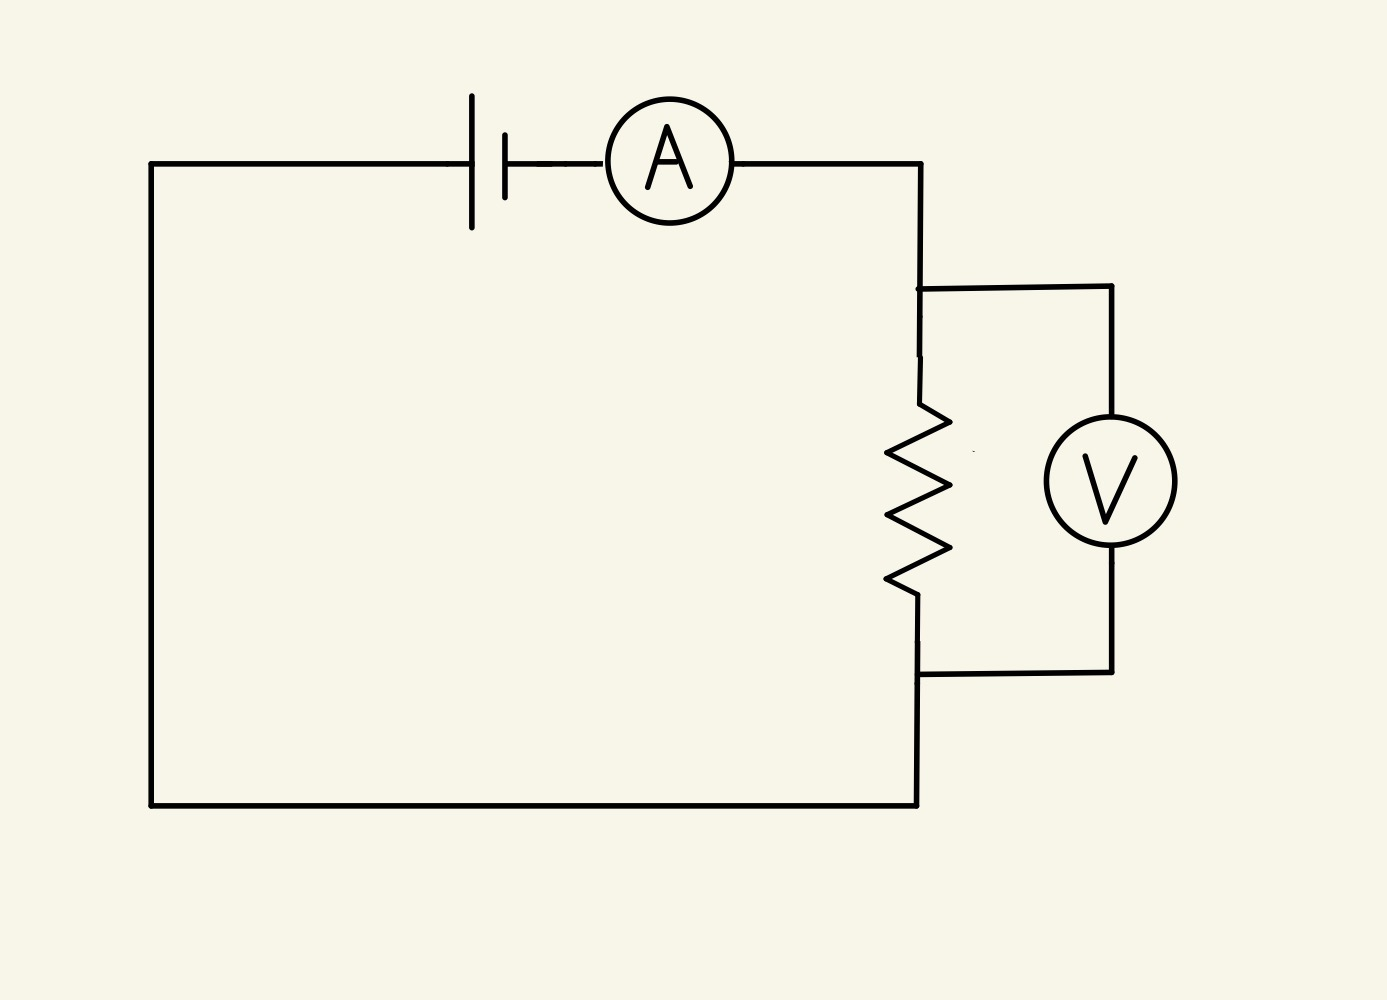
\includegraphics[width=0.3\textwidth]{experimentOneApparatus}&
	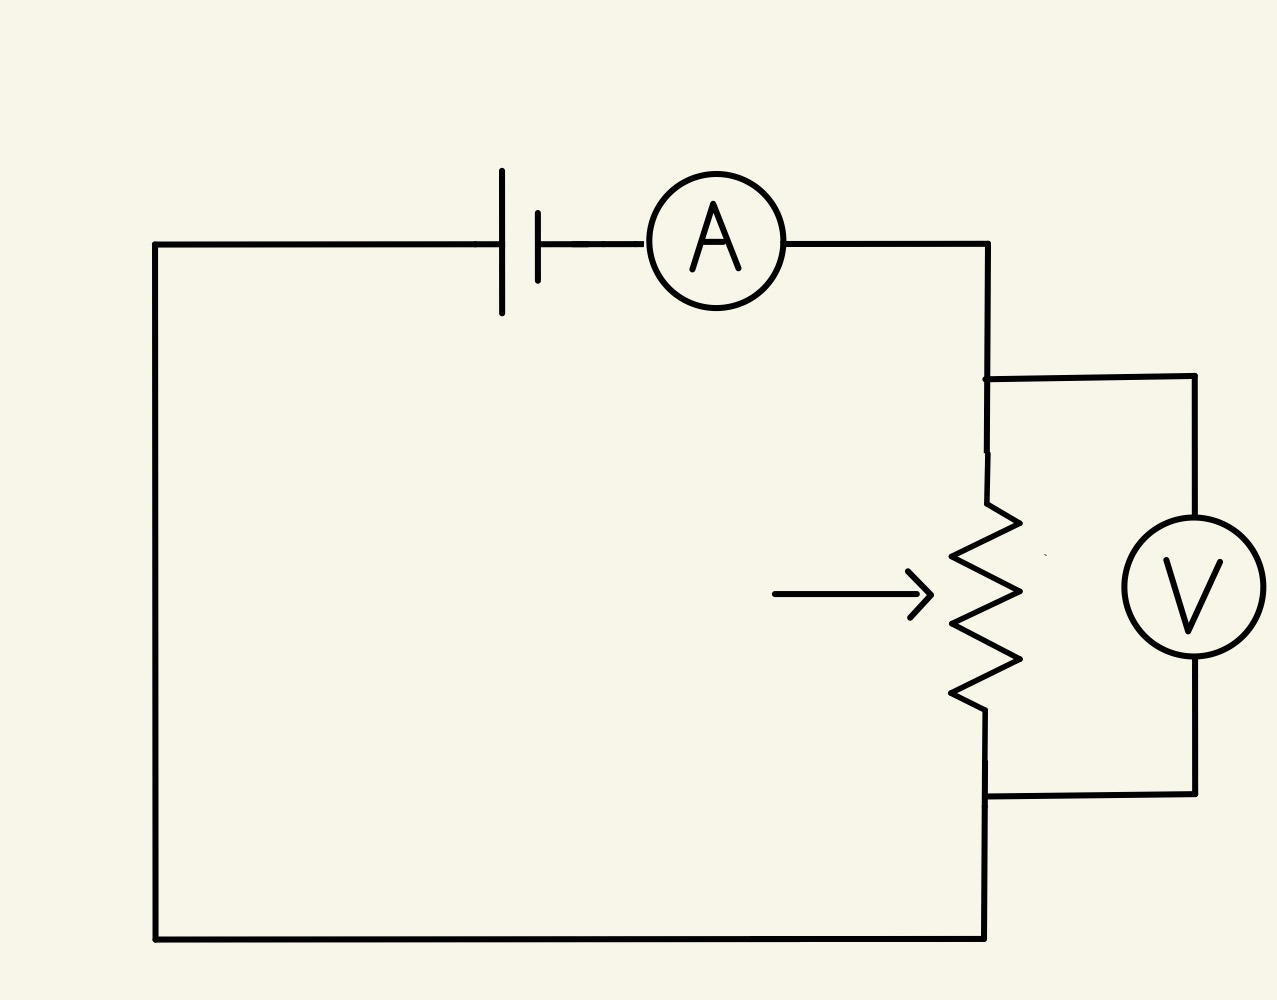
\includegraphics[width=0.3\textwidth]{experimentTwoApparatus}&
	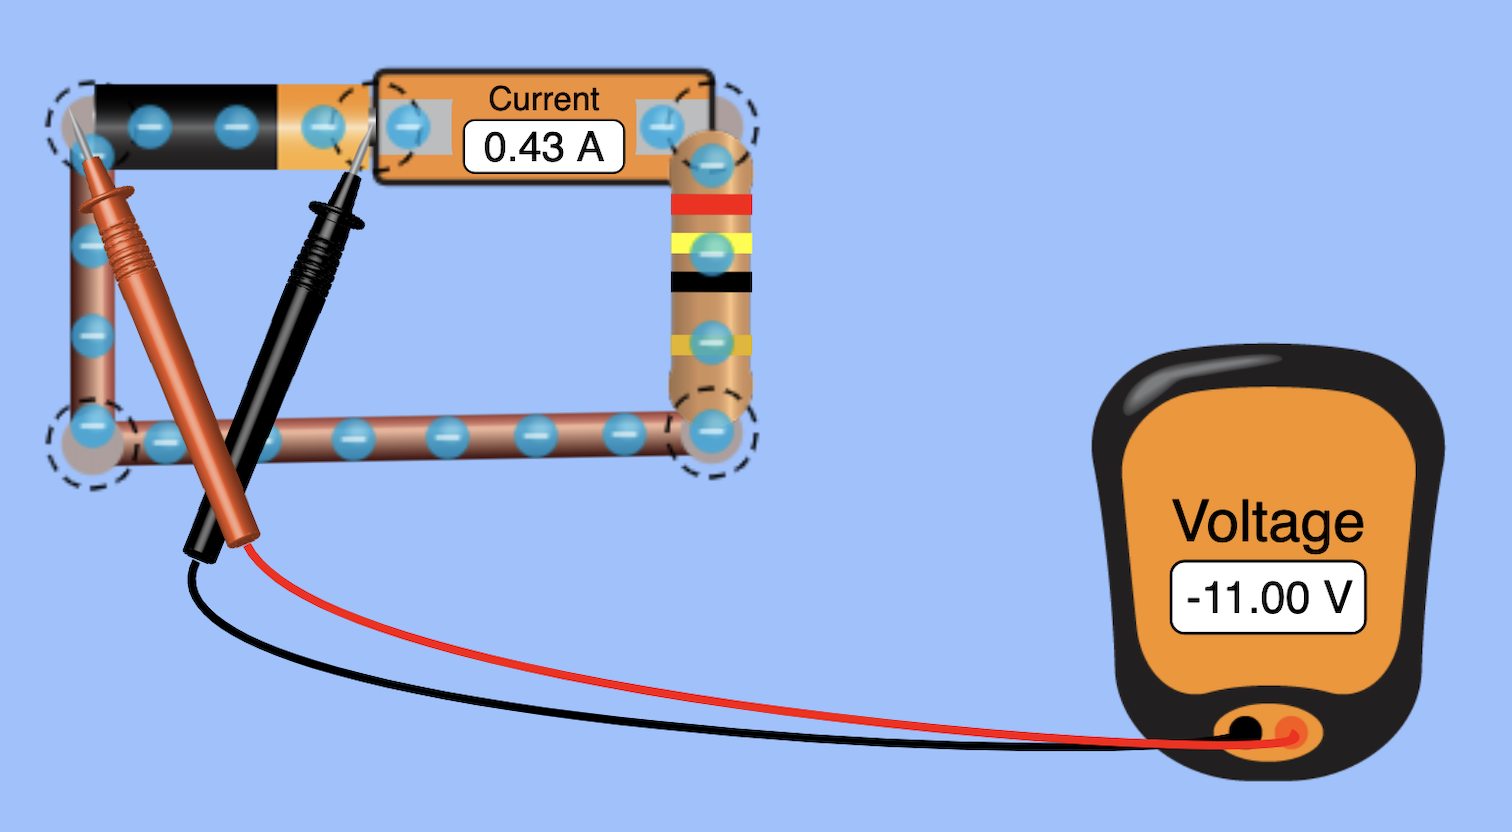
\includegraphics[width=0.3\textwidth]{experimentThreeApparatus}\\
	\textbf{Figure 2.1:}&
	\textbf{Figure 2.2:}&
	\textbf{Figure 2.3:}\\
	\textbf{Experiment 1 Apparatus}&
	\textbf{Experiment 2 Apparatus}&
	\textbf{Experiment 3 Apparatus}
\end{tabular}
\end{center}
\section{Results}
{\large\textbf{Uncertainty Calculation}}
{\vspace{5pt}}\\
All uncertainty calculations are based on the data available in the \textbf{U1270 Series Handheld Digital Multimeter} manual. All uncertainty
	calculations for this multimeter are calculated as a percentage of the value plus a count of the least significant digit. This is mathematically
	represented by \textbf{Function 4.1}. This formula was then used to create \textbf{Function 4.1} (\lstinline{calculate_uncertainty()}) which was
	used for all uncertainty calculations of the multimeter data in the graphs and data tables.\\
Sample uncertainty calculations are shown in the appendix under \textbf{Sample uncertainty calculations}.
{\vspace{10pt}}\\
{\large\textbf{Curve Fitting}}
{\vspace{5pt}}\\
\textbf{Experiments 1 \& 2}\\
To determine the resistance and its uncertainty of the resistor and potentiometer from the experimental data sets, \textbf{Function 4.2} was
	defined and passed into the \lstinline{scipy.optimize} module's \lstinline{curve_fit} function for each experiment. The slopes of the linear model, as shown in \textbf{Figure 3.1}
	and \textbf{Figure 3.2}, represent the reciprocal of the value for resistance. Thus taking the reciprocal of the slope and multiplying it by 1000, as
	the current was measured in milliamps, provided the value of resistance for the resistor and potentiometer which were determined to be
	$467.9 \pm 0.1 \Omega$ and $7559 \pm 1 \Omega$ respectively. The uncertainty was determined by using the error propagation equation for division (\textbf{Function 4.5}),
	as the reciprocal of the slope had to be taken, and then multiplied by $1000$ to determine the uncertainty in ohms.\\

For experiment 1, the value of resistance was also determined using the coloured bands found on the resistor. \textbf{Figure 5.1} in the
	appendix details the resistance colour codes. For experiment 1, the bands were observed to be yellow, violet, black and gold.
	This corresponds to a value of $470 \pm 20 \Omega$.
\vspace{5pt}\\
\textbf{Experiment 3}\\
To determine the value of the experimental exponents, coefficients and their uncertainties in experiment 3, \textbf{Function 4.2} and \textbf{Function 4.3}
	were used for linear and nonlinear modelling respectively and the values were solved for using \lstinline{curve_fit}.
	Note, the linear regression was performed on the voltage and current after the logarithm of the data was taken. The fitted exponents determined using
	the linear and nonlinear models were determined to be $0.44 \pm 0.01$
	and $0.47 \pm 0.01$ respectively. The coefficients determined using the linear and nonlinear models were determined to be $7.4 \pm 0.1$ and
	$7.0 \pm 0.2$ respectively. Thus, the power law relations determined from the linear and nonlinear models were $ I = 7.4 V ^ {0.44}$ and
	$I = 7.0 V ^{0.47}$. Note, the error propagation equation for exponential functions (\textbf{Function 4.6}) was used to determine the uncertainty value of the coefficient
	from the linear model as the value of the coefficient from the linear model had to be exponentiated. Similarly to determine the coefficient for the
	theoretical curve, the \lstinline{model_light()} model (\textbf{Function 4.4}), which uses $0.6$ as its fitted exponent, was passed into the \lstinline{curve_fit()} function.
	The coefficient was determined to be $4.6$.
{\vspace{10pt}}\\
{\large\textbf{Chi-squared calculations}}
{\vspace{5pt}}\\
The function \lstinline{calculatechisquared()} (\textbf{Function 4.7}) was used. For experiments 1 and 2, the respective reduced chi-squared values calculated were
	$0.609$, $0.007$ and $41.469$ and $35.186$ for the linear and nonlinear models in experiment 3 respectively.\\

{\large\textbf{Final Graphs}}
{\vspace{5pt}}\\
Note, all the following graphs were generated with Python.\\
\begin{center}
	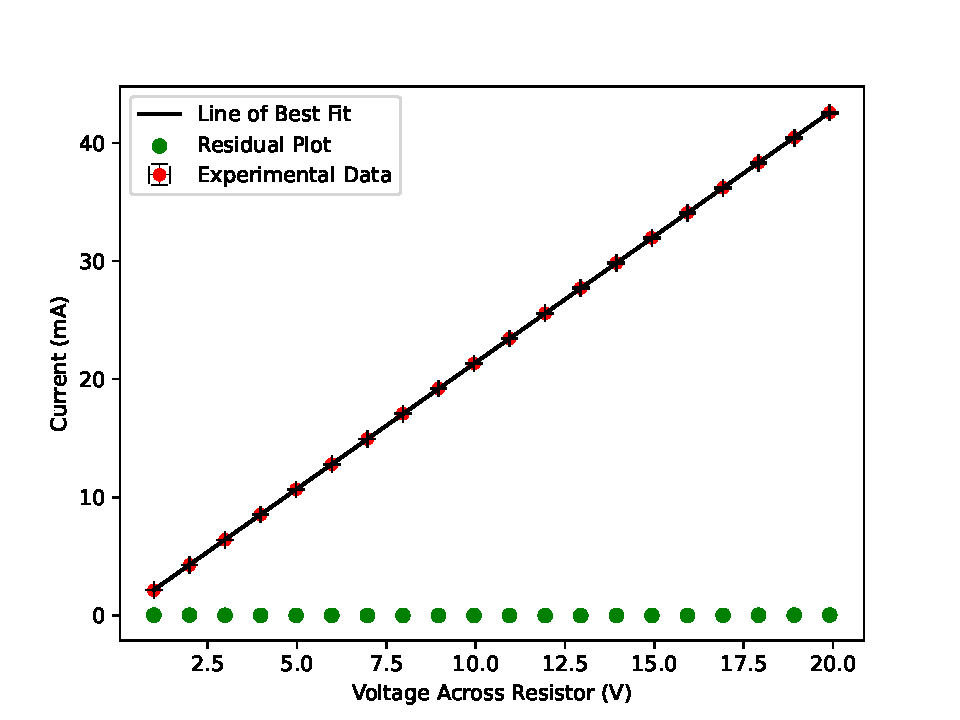
\includegraphics[width=0.65\textwidth]{experimentOne}
\end{center}
\begin{center}
    \textbf{Figure 3.1: A plot of the data collected in experiment 1 demonstrating the relationship between the potential difference and current. The slope of the line of best fit represents the reciprocal of the resistance value of the resistor.}\\
\end{center}
\begin{center}
	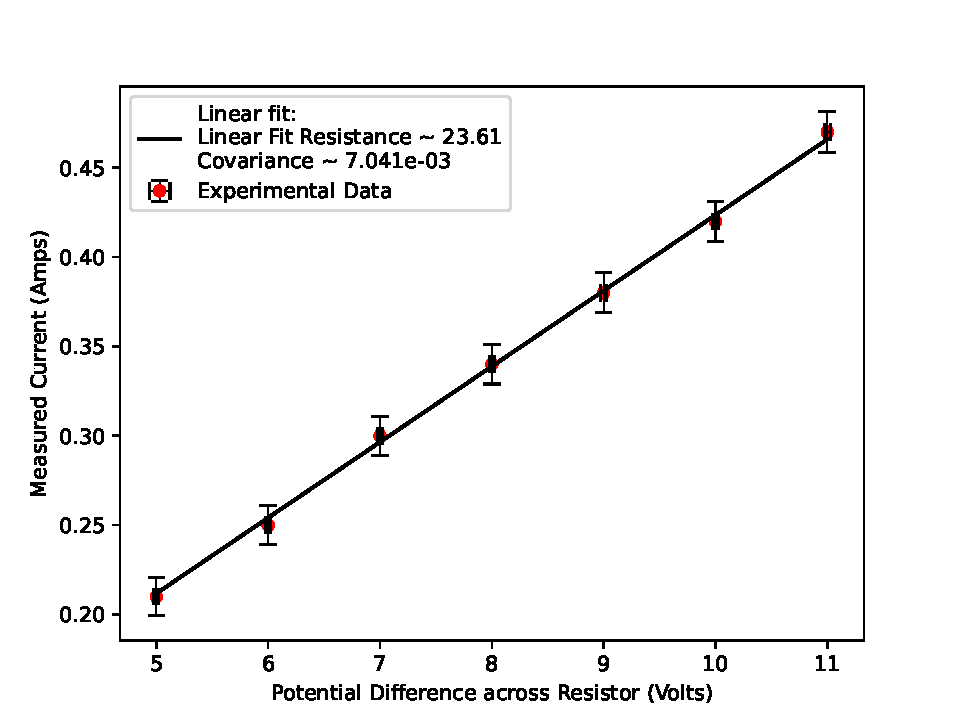
\includegraphics[width=0.65\textwidth]{experimentTwo}
\end{center}
\begin{center}
    \textbf{Figure 3.2: A plot of the data collected in experiment 2 demonstrating the relationship between the potential difference and current. The slope of the line of best fit represents the reciprocal of the resistance value of the resistor.}\\
\end{center}
\begin{center}
	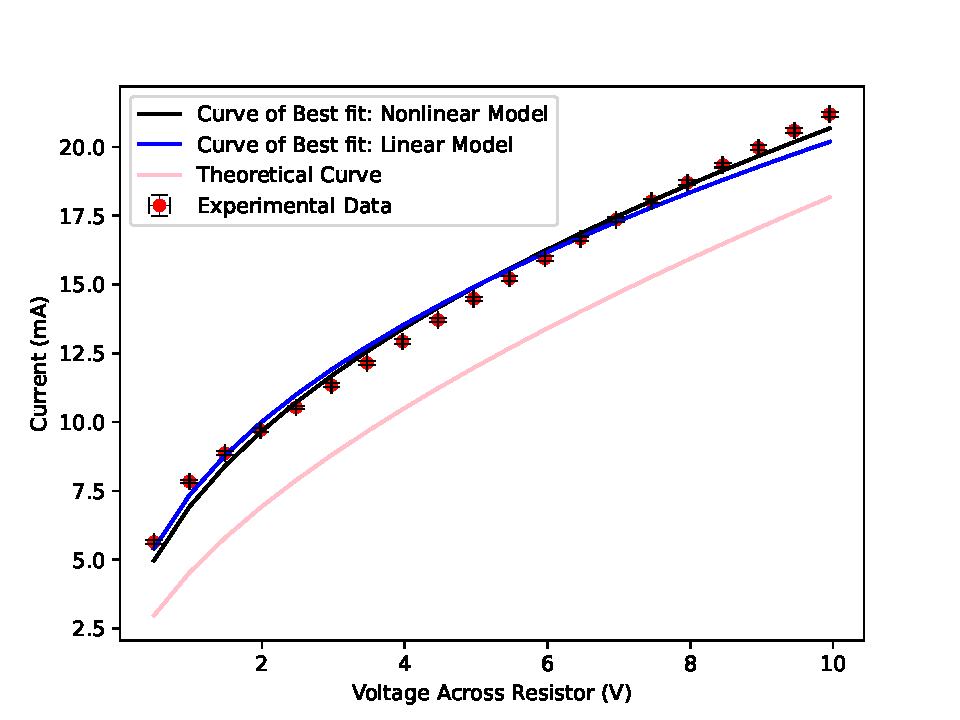
\includegraphics[width=0.65\textwidth]{experimentThreeOne}
\end{center}
\begin{center}
    \textbf{Figure 3.3: A plot of the data collected in experiment 3 demonstrating the relationship between the potential difference across the lightbulb and current through the circuit. Contains three best fit lines: the nonlinear model of the raw data, the linear model of the linearized data and a theoretical curve based on tungsten equation.}\\
\end{center}
\begin{center}
	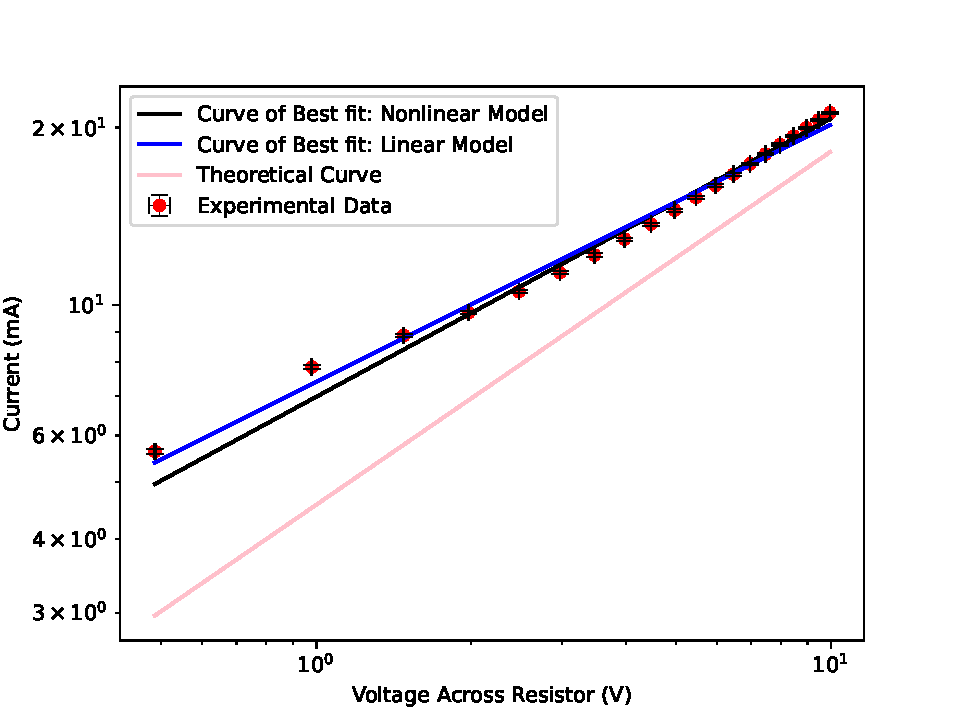
\includegraphics[width=0.65\textwidth]{experimentThreeTwo}
\end{center}
\begin{center}
    \textbf{Figure 3.4: A linearized plot of the data collected in experiment 3 demonstrating the relationship between the potential difference across the lightbulb and current through the circuit. Contains three best fit lines: the nonlinear model of the raw data, the linear model of the linearized data and a theoretical curve based on tungsten equation.}\\
\end{center}
\newpage
\section{Analysis and Discussion} % #4
In regards to experiments 1 and 2, the experimental resistance values were very close to the expected values of $470 \Omega$ and $7579 \Omega$.
Examining the graphs generated for each experiment, the line of best fit did not pass through zero.
However, since the experiments were not conducted under perfect conditions, it is likely that the readings for the currents and
	voltages deviated from their expected values and in turn, would force the line of best fit to not pass through zero.
Forcing the line of best fit to pass through zero yields resistance values of $467.4 \Omega$ and $7575.2 \Omega$. Analyzing the quality
	of fit of the linear model for experiment 1, the reduced chi-squared value was roughly 0.609. Although the reduced chi-squared
	value was not much less than 1, this still indicates that the uncertainties may have been overestimated, however,
	the calculation for the uncertainty in the current came from the Keysight-U1272 manual. In regards to experiment 2,
	the reduced chi-squared value computed was roughly 0.007. In this case, the reduced chi-squared value was significantly
	less than 1. Similarly to experiment 1, this may have resulted from an overestimate of the uncertainty in the current, however,
	the calculation for the uncertainty came from the Keysight-U1272 manual. In both cases, since the values were less than 1 this indicates that the linear model was over-fit.\\

Analyzing experiment 3, the experimental exponents were determined to be $0.44 \pm 0.01$ using the linear model, and $0.47 \pm 0.01$
	using the nonlinear model. The nonlinear model ultimately gave an exponent closer to the expected value of 0.6.
Examining \textbf{Figure 3.3} and \textbf{Figure 3.4}, the nonlinear model is visually a better fit for the measured data, however, both experimental
	exponent values do not fall within the range of the blackbody value, $0.6$. In comparison to the expected value for the tungsten,
	0.663, the experimental exponents deviate even further. Analyzing the quality of fit of the nonlinear model, the value of the
	reduced chi-squared was computed to be 35.186 which is significantly greater than 1. Examining \textbf{Figure 3.3}, the line of best fit using
	the nonlinear regression method tends to deviate significantly away from some of the measured data points. It follows that the difference
	between the measured and predicted values would be larger. Although the uncertainty in the current was determined using the Keysight-U1272 manual,
	they were quite small. Thus, these two factors are likely to have resulted in the reduced chi-squared value being significantly larger than the accepted value of 1.\\

In regards to the linear model, the reduced chi-squared value was determined to be 41.469 which is also significantly greater than 1.
For similar reasoning as in the nonlinear model, the large difference between the predicted and measured data and the small current uncertainties were
likely to have contributed to the large reduced chi-squared value. Thus it follows that although the nonlinear model was determined to have a smaller
reduced chi-squared value, the reduced chi-squared values for both models indicate that they are a poor fit for the experimental data.\\

In regards to experiments 1 and 2, it follows that the experimental results ultimately verify that the resistance of the resistor and potentiometer
	can be quantified using Ohm’s law, however, it must be noted that with their uncertainties, both experimental values fall slightly below the expected values.
This may be due to the added resistance in the wires and temperature fluctuations in the resistor and potentiometer affecting the current and voltage readings.
Although in the case of experiment 1, the experimental resistance value does fall within the range of the resistance value calculated using the color bands on the resistor.
Reviewing experiment 3, although the experimental results do not agree with the theoretical power law, added resistance in the wires and temperature fluctuations
	due to the light bulb within the circuit similarly may have caused error in the collection of the experimental data.

\newpage
\section{Appendix}
{\large \textbf{Tables}}\\
\begin{center}
	\begin{tabular}{ | l | l | l | }
		\hline
		Voltage Across Battery&Current& Voltage Across Resistor\\
		($V$) & ($mA$) & ($V$)\\
		 & & \\
		\hline
		$1.000$&$2.131\pm0.009$&$0.994\pm0.002$\\
		$2.000$&$4.265\pm0.01$&$1.99\pm0.003$\\
		$3.000$&$6.397\pm0.02$&$2.984\pm0.003$\\
		$4.000$&$8.531\pm0.02$&$3.98\pm0.004$\\
		$5.000$&$10.665\pm0.03$&$4.975\pm0.004$\\
		$6.000$&$12.799\pm0.03$&$5.971\pm0.005$\\
		$7.000$&$14.933\pm0.03$&$6.967\pm0.005$\\
		$8.000$&$17.065\pm0.04$&$7.963\pm0.006$\\
		$9.000$&$19.197\pm0.04$&$8.958\pm0.006$\\
		$10.000$&$21.32\pm0.05$&$9.954\pm0.007$\\
		$11.000$&$23.45\pm0.05$&$10.95\pm0.007$\\
		$12.000$&$25.58\pm0.06$&$11.946\pm0.008$\\
		$13.000$&$27.71\pm0.06$&$12.941\pm0.008$\\
		$14.000$&$29.83\pm0.06$&$13.937\pm0.009$\\
		$15.000$&$31.96\pm0.07$&$14.932\pm0.009$\\
		$16.000$&$34.08\pm0.07$&$15.928\pm0.01$\\
		$17.000$&$36.2\pm0.08$&$16.924\pm0.01$\\
		$18.000$&$38.32\pm0.08$&$17.92\pm0.01$\\
		$19.000$&$40.44\pm0.09$&$18.916\pm0.01$\\
		$20.000$&$42.56\pm0.09$&$19.911\pm0.01$\\
		\hline
	\end{tabular}
\end{center}
\begin{center}
    \textbf{Table 4.1: Experiment 1 Raw Data}\\
\end{center}

\begin{center}
	\begin{tabular}{ | l | l | l | }
		\hline
		Voltage Across Battery&Current& Voltage Across Potentiometer\\
		($V$) & ($mA$) & ($V$)\\
		 & & \\
		\hline
		$1.000$&$0.129\pm0.005$&$0.999\pm0.002$\\
		$2.000$&$0.261\pm0.006$&$1.999\pm0.003$\\
		$3.000$&$0.393\pm0.006$&$2.997\pm0.003$\\
		$4.000$&$0.525\pm0.006$&$3.997\pm0.004$\\
		$5.000$&$0.658\pm0.006$&$4.997\pm0.004$\\
		$6.000$&$0.789\pm0.007$&$5.998\pm0.005$\\
		$7.000$&$0.922\pm0.007$&$6.997\pm0.005$\\
		$8.000$&$1.054\pm0.007$&$7.998\pm0.006$\\
		$9.000$&$1.186\pm0.007$&$8.998\pm0.006$\\
		$10.000$&$1.318\pm0.008$&$9.998\pm0.007$\\
		$11.000$&$1.45\pm0.008$&$10.998\pm0.007$\\
		$12.000$&$1.583\pm0.008$&$11.998\pm0.008$\\
		$13.000$&$1.715\pm0.008$&$12.998\pm0.008$\\
		$14.000$&$1.847\pm0.009$&$13.998\pm0.009$\\
		$15.000$&$1.98\pm0.009$&$14.996\pm0.009$\\
		$16.000$&$2.113\pm0.009$&$15.997\pm0.01$\\
		$17.000$&$2.245\pm0.009$&$16.998\pm0.01$\\
		$18.000$&$2.377\pm0.01$&$17.998\pm0.01$\\
		$19.000$&$2.51\pm0.01$&$18.998\pm0.01$\\
		$20.000$&$2.643\pm0.01$&$19.998\pm0.01$\\
		\hline
	\end{tabular}
\end{center}
\begin{center}
    \textbf{Table 4.2: Experiment 2 Raw Data}\\
\end{center}


\begin{center}
	\begin{tabular}{ | l | l | l | }
		\hline
		Voltage Across Battery&Current& Voltage Across Light Bulb\\
		($V$) & ($mA$) & ($V$)\\
		 & & \\
		\hline
		$1.000$&$5.64\pm0.06$&$0.486\pm0.002$\\
		$2.000$&$7.84\pm0.07$&$0.981\pm0.002$\\
		$3.000$&$8.87\pm0.07$&$1.479\pm0.003$\\
		$4.000$&$9.7\pm0.07$&$1.977\pm0.003$\\
		$5.000$&$10.53\pm0.07$&$2.475\pm0.003$\\
		$6.000$&$11.34\pm0.07$&$2.973\pm0.003$\\
		$7.000$&$12.15\pm0.07$&$3.471\pm0.004$\\
		$8.000$&$12.93\pm0.08$&$3.97\pm0.004$\\
		$9.000$&$13.71\pm0.08$&$4.468\pm0.004$\\
		$10.000$&$14.48\pm0.08$&$4.967\pm0.004$\\
		$11.000$&$15.22\pm0.08$&$5.466\pm0.005$\\
		$12.000$&$15.95\pm0.08$&$5.964\pm0.005$\\
		$13.000$&$16.66\pm0.08$&$6.463\pm0.005$\\
		$14.000$&$17.35\pm0.08$&$6.961\pm0.005$\\
		$15.000$&$18.03\pm0.09$&$7.46\pm0.006$\\
		$16.000$&$18.7\pm0.09$&$7.959\pm0.006$\\
		$17.000$&$19.34\pm0.09$&$8.458\pm0.006$\\
		$18.000$&$19.97\pm0.09$&$8.956\pm0.006$\\
		$19.000$&$20.59\pm0.09$&$9.455\pm0.007$\\
		$20.000$&$21.19\pm0.09$&$9.954\pm0.007$\\
		\hline
	\end{tabular}
\end{center}
\begin{center}
    \textbf{Table 4.3: Experiment 1 Raw Data}\\
\end{center}

\begin{center}
	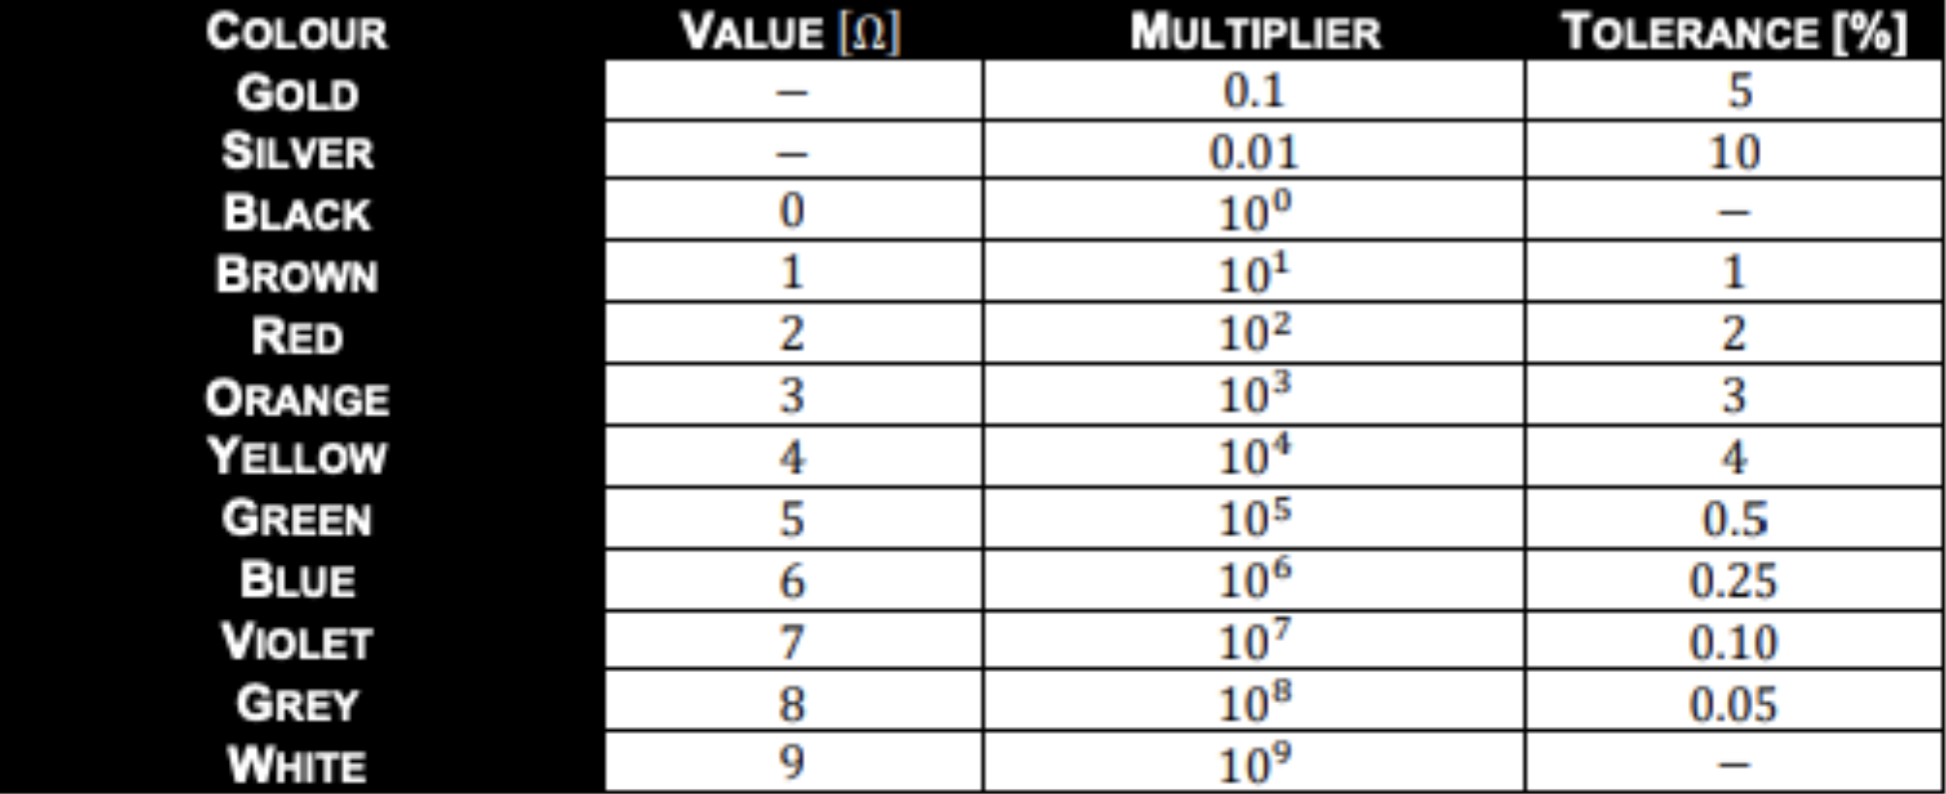
\includegraphics[width=1\textwidth]{resistorBandTable}
\end{center}
\begin{center}
    \textbf{Table 4.4: A table detailing the resistance colour codes.}\\
\end{center}

\newpage

{\large\textbf{Uncertainty}}
{\vspace{10pt}}\\
$$ u(x) = \pm\left|\frac{xp}{100} + c r\right|$$
\begin{center}
    \textbf{Function 4.1: Uncertainty calculation formula.}\\
\end{center}
Values corresponding to the multimter setting used are obtained from the \textbf{U1270 Series Handheld Digital Multimeter} manual:\\
- $p$: Percentage of the reading\\
- $r$: Resolution / Least Significant Digit\\
- $c$: Count of Least Significant Digit\\
\vspace{10pt}
\begin{verbatim}
def calculate_uncertainty(value, res, percentage, multiplier):
    return value * percentage / 100 + res * multiplier
\end{verbatim}
\begin{center}
    \textbf{Function 4.1: Function used to calculate uncertainty for all values (implementation of Equation 4.1).}\\
\end{center}
{\vspace{10pt}}
{\large\textbf{Equations and Functions}}
$$f(x) = ax + b$$
\begin{center}
	\textbf{Equation 4.2: Generic linear equation}
\end{center}
\begin{verbatim}
def linear_model(values, a, b):
    return a * values + b
\end{verbatim}
\begin{center}
    \textbf{Function 4.2: Model used for linear curve fitting (implementation of Equation 4.2)}\\
\end{center}

$$f(x) = ax^b$$
\begin{center}
	\textbf{Equation 4.3: Generic exponential function}
\end{center}
\begin{verbatim}
def nonlinear_model(values, a, b):
    return a * values ** b
\end{verbatim}
\begin{center}
    \textbf{Function 4.3: Model used for nonlinear curve fitting.}\\
\end{center}

$$f(x) = ax^{\frac35}$$
\begin{center}
	\textbf{Equation 4.4: Theoretical model}
\end{center}
\newpage
\begin{verbatim}
def model_light(a, values):
    return a * values ** (3 / 5)
\end{verbatim}
\begin{center}
	\textbf{Function 4.4: Model used for experiment 3 theoretical curve  (implementation of Equation 4.4)}\\
\end{center}

$$u\left(\frac ab\right) = \frac{a\times u(a)}{b}$$
\begin{center}
	\textbf{Equation 4.5: Division error propagation equation}
\end{center}
\begin{verbatim}
def error_propagation_division(value1, value2, uncertainty):
    return value1 * uncertainty / value2
\end{verbatim}
\begin{center}
    \textbf{Function 4.5: Division error propagation function (implementation of Equation 4.5)}\\
\end{center}


$$u(a^x) = x u(x)$$
\begin{center}
	\textbf{Equation 4.6: Exponential error propagation equation}
\end{center}
\begin{verbatim}
def error_propagation_exponential(value, uncertainty):
    return value * uncertainty
\end{verbatim}
\begin{center}
    \textbf{Function 4.6: Exponential error propagation function (implementation of Equation 4.6)}\\
\end{center}

$$ \chi^2_r = \frac{1}{v}\sum^{n}_{i=1}{\left(\frac{y_i - y(x_i)}{u(y_i)}\right)^2}$$
\begin{center}
	\textbf{Equation 4.7: Reduced chi squared equation}
\end{center}

\begin{verbatim}
def calculatechisquared(
    xvalues, yvalues, yuncertainty, model, *modelparameters
):
    return (1 / (len(xvalues) - len(modelparameters))) * np.sum(
        ((yvalues - model(xvalues, *modelparameters)) / yuncertainty) ** 2
    )
\end{verbatim}
\begin{center}
\textbf{Function 4.7: Function used to calculate reduced chi squared values (implementation of Equation 4.7)}
\end{center}
\vspace{20pt}
\newpage
{\Large\textbf{Sample uncertainty calculations}}\\

\textbf{Voltmeter Calculation sample for $30V$ setting}\\
Using \textbf{Function 4.1}, the corresponding values for $30V$ are:\\
$r = 0.001$, $p = 0.05$, $c=2$ (from the voltmeter manual)\\
Let $V_i$ represent an arbitrary voltage measurement made with the $30V$ setting.\\
$$u(V_i) = \pm \left|\frac{0.05V_i }{100} +  2* 0.001\right|V = \pm\left|0.0005V_i + 0.002\right|V$$
For example in experiment 1, the first measured voltage was: $V_1=0.994$\\
$$u(V_1) = \pm \left|0.0005 \times 0.994 + 0.002\right|V \approx \pm 0.002497V$$\\
\textbf{Ammeter Calculation sample for $30mA$ setting}\\
Using \textbf{Function 4.1}, the corresponding values for $30mA$ are:\\
$r = 0.001$, $p = 0.2$, $c=5$ (from the ammeter manual)\\
Let $I_i$ represent an arbitrary current measurement made with the $30mA$ setting.\\
$$u(I_i) = \pm \left|\frac{0.2I_i }{100} +  5* 0.001\right|mA = \pm\left|0.002I_i + 0.005\right|mA$$
For example in experiment one, the measured current was: $I_1 = 2.131mA$.
$$u(I_1)= u(2.131) = \pm\left|0.002 \times 2.131 + 0.005\right|mA \approx \pm 0.009262mA$$\\
\end{document}